%%%%%%%%%%%%%%%%%%%%%%%%%%%%%%%%%%%%%%%%%%%%%%%%%%%%%%%%%%%%%%%%%%%%%
%%                                                                 %%
%% Please do not use \input{\dots} to include other tex files.       %%
%% Submit your LaTeX manuscript as one .tex document.              %%
%%                                                                 %%
%% All additional figures and files should be attached             %%
%% separately and not embedded in the \TeX\ document itself.       %%
%%                                                                 %%
%%%%%%%%%%%%%%%%%%%%%%%%%%%%%%%%%%%%%%%%%%%%%%%%%%%%%%%%%%%%%%%%%%%%%

%%\documentclass[referee,sn-basic]{sn-jnl}% referee option is meant for double line spacing

%%=======================================================%%
%% to print line numbers in the margin use lineno option %%
%%=======================================================%%

%%\documentclass[lineno,sn-basic]{sn-jnl}% Basic Springer Nature Reference Style/Chemistry Reference Style

%%======================================================%%
%% to compile with pdflatex/xelatex use pdflatex option %%
%%======================================================%%

%%\documentclass[pdflatex,sn-basic]{sn-jnl}% Basic Springer Nature Reference Style/Chemistry Reference Style

%%\documentclass[sn-basic]{sn-jnl}% Basic Springer Nature Reference Style/Chemistry Reference Style
\documentclass[sn-mathphys]{sn-jnl}% Math and Physical Sciences Reference Style
%%\documentclass[sn-aps]{sn-jnl}% American Physical Society (APS) Reference Style
%%\documentclass[sn-vancouver]{sn-jnl}% Vancouver Reference Style
%%\documentclass[sn-apa]{sn-jnl}% APA Reference Style
%%\documentclass[sn-chicago]{sn-jnl}% Chicago-based Humanities Reference Style
%%\documentclass[sn-standardnature]{sn-jnl}% Standard Nature Portfolio Reference Style
%%\documentclass[default]{sn-jnl}% Default
%%\documentclass[default,iicol]{sn-jnl}% Default with double column layout

%%%% Standard Packages
%%<additional latex packages if required can be included here>
%%%%

%%%%%=============================================================================%%%%
%%%%  Remarks: This template is provided to aid authors with the preparation
%%%%  of original research articles intended for submission to journals published
%%%%  by Springer Nature. The guidance has been prepared in partnership with
%%%%  production teams to conform to Springer Nature technical requirements.
%%%%  Editorial and presentation requirements differ among journal portfolios and
%%%%  research disciplines. You may find sections in this template are irrelevant
%%%%  to your work and are empowered to omit any such section if allowed by the
%%%%  journal you intend to submit to. The submission guidelines and policies
%%%%  of the journal take precedence. A detailed User Manual is available in the
%%%%  template package for technical guidance.
%%%%%=============================================================================%%%%

\jyear{2023}%

%% as per the requirement new theorem styles can be included as shown below
\theoremstyle{thmstyleone}%
\newtheorem{theorem}{Theorem}%  meant for continuous numbers
%%\newtheorem{theorem}{Theorem}[section]% meant for sectionwise numbers
%% optional argument [theorem] produces theorem numbering sequence instead of independent numbers for Proposition
\newtheorem{proposition}[theorem]{Proposition}%
%%\newtheorem{proposition}{Proposition}% to get separate numbers for theorem and proposition etc.

\theoremstyle{thmstyletwo}%
\newtheorem{example}{Example}%
\newtheorem{remark}{Remark}%

\theoremstyle{thmstylethree}%
\newtheorem{definition}{Definition}%

\raggedbottom
%%\unnumbered% uncomment this for unnumbered level heads

% JAIME: this is to hide font size warnings
\usepackage{anyfontsize}

% JAIME: For 1e-10 notation
\usepackage{siunitx}


\begin{document}

\title[Predicting Spotify Audio Features from Last.fm Tags]{Predicting Spotify Audio Features from Last.fm Tags}

%%=============================================================%%
%% Prefix	-> \pfx{Dr}
%% GivenName	-> \fnm{Joergen W.}
%% Particle	-> \spfx{van der} -> surname prefix
%% FamilyName	-> \sur{Ploeg}
%% Suffix	-> \sfx{IV}
%% NatureName	-> \tanm{Poet Laureate} -> Title after name
%% Degrees	-> \dgr{MSc, PhD}
%% \author*[1,2]{\pfx{Dr} \fnm{Joergen W.} \spfx{van der} \sur{Ploeg} \sfx{IV} \tanm{Poet Laureate}
%%                 \dgr{MSc, PhD}}\email{iauthor@gmail.com}
%%=============================================================%%



\author*[1]{\fnm{Jaime} \sur{Ramírez Castillo}}\email{Jaime.Ramirez@alu.uclm.es}
\equalcont{These authors contributed equally to this work.}

\author[1]{\fnm{M. Julia} \sur{Flores}}\email{Julia.Flores@uclm.es}
\equalcont{These authors contributed equally to this work.}

\author[2]{\fnm{Philippe} \sur{Leray}}\email{philippe.leray@univ-nantes.fr}

\affil*[1]{\orgdiv{Departamento de Sistemas Informáticos}, \orgname{Universidad de Castilla-La Mancha}, \orgaddress{\street{Campus universitario s/n}, \city{Albacete}, \postcode{02071}, \country{Spain}}}

\affil[2]{\orgdiv{Laboratoire des Sciences du Numérique de Nantes}, \orgname{Centre national de la recherche scientifique, University of Nantes}, \orgaddress{\city{Nantes}, \country{France}}}


%%==================================%%
%% sample for unstructured abstract %%
%%==================================%%

\abstract{
      Music information retrieval (MIR) is an interdisciplinary research field that focuses on the extraction, processing,
      and knowledge discovery of information contained in music.
      While previous studies have utilized Spotify audio features
      and Last.fm tags as input values for classification tasks, such as music genre recognition,
      their potential as target values has remained unexplored.
      In this article, we address this notable gap in the research landscape by proposing a novel approach to predict
      Spotify audio features based on a set of Last.fm tags.
      By predicting audio features, we aim to explore the relationship between subjective perception and concrete musical features,
      shedding light on patterns and hidden correlations between how music is perceived, consumed, and discovered.
      Additionally, the predicted audio features can be leveraged in recommendation systems
      to provide users with explainable recommendations, bridging the gap between algorithmic suggestions and user understanding.
      Our experiments involve training models such as GPT-2, XGBRegressor, and Bayesian Ridge regressor to predict
      Spotify audio features from Last.fm tags.
      Through our findings, we contribute to the advancement of MIR research by demonstrating the potential of Last.fm
      tags as target values and paving the way for future research on the connection between subjective and objective music characterization.
      Our approach holds promise for both listeners and researchers,
      offering new insights into the intricate relationship between perception and audio signal in music.
}


% TENSES: https://blog.wordvice.com/video-which-verb-tenses-should-i-use-in-a-research-paper/

%%================================%%
%% Sample for structured abstract %%
%%================================%%

% \abstract{\textbf{Purpose:} The abstract serves both as a general introduction to the topic and as a brief, non-technical summary of the main results and their implications. The abstract must not include subheadings (unless expressly permitted in the journal's Instructions to Authors), equations or citations. As a guide the abstract should not exceed 200 words. Most journals do not set a hard limit however authors are advised to check the author instructions for the journal they are submitting to.
%
% \textbf{Methods:} The abstract serves both as a general introduction to the topic and as a brief, non-technical summary of the main results and their implications. The abstract must not include subheadings (unless expressly permitted in the journal's Instructions to Authors), equations or citations. As a guide the abstract should not exceed 200 words. Most journals do not set a hard limit however authors are advised to check the author instructions for the journal they are submitting to.
%
% \textbf{Results:} The abstract serves both as a general introduction to the topic and as a brief, non-technical summary of the main results and their implications. The abstract must not include subheadings (unless expressly permitted in the journal's Instructions to Authors), equations or citations. As a guide the abstract should not exceed 200 words. Most journals do not set a hard limit however authors are advised to check the author instructions for the journal they are submitting to.
%
% \textbf{Conclusion:} The abstract serves both as a general introduction to the topic and as a brief, non-technical summary of the main results and their implications. The abstract must not include subheadings (unless expressly permitted in the journal's Instructions to Authors), equations or citations. As a guide the abstract should not exceed 200 words. Most journals do not set a hard limit however authors are advised to check the author instructions for the journal they are submitting to.}

\keywords{Music information retrieval, Artificial intelligence}

%%\pacs[JEL Classification]{D8, H51}

%%\pacs[MSC Classification]{35A01, 65L10, 65L12, 65L20, 65L70}

\maketitle

\section{Introduction}\label{sec1}

Music information retrieval (MIR) is an interdisciplinary research field that encompasses the extraction,
processing, and knowledge discovery of information contained in music.
MIR research covers a wide range of applications and intersects with other areas, such as computer science, signal processing, musicology, and sociology.
Examples of MIR applications are recommendation systems, music classification,
music source separation, and music generation, among others \cite{ramirez2020machine}.

MIR applications often attempt to extract information from the music audio signal,
although analyzing associated metadata is also a common practice.
Audio signals are typically preprocessed and transformed into intermediate formats, such as frequency-based signal representations (e.g. spectrograms),
and sets of hand-crafted audio features, which are typically engineered by using domain knowledge (e.g. MFCC, rhythm, or tonal descriptors).

The metadata associated to a music piece is available in multiple formats.
Editorial information or lyrics, for example, are mostly available in text format.
The ability to process images or videos might be also required, for example, for analyzing album artwork, or music videos.

Depending on the specific MIR application, researchers and practitioners create models that generate different output values.
Applications that extract audio features typically return audio descriptors, namely values related to the tempo, the key, or the sample rate, to name a few.
Open source libraries such as \emph{Librosa}\footnote[1]{https://librosa.org/}
and \emph{Essentia}\footnote[2]{https://essentia.upf.edu/index.html} offer methods to extract these values.
Other applications might produce more abstract or subjective values, for example, by using machine learning techniques
that estimate the emotion that a track induces, or the music genre of this track.

Among potentially useful input and output values, research has proved \emph{Spotify audio features} and \emph{Last.fm tags} to be significant values used to  characterize music.
Spotify audio features capture high-level information about the music signal and how humans perceive this signal.
Examples of these features are such as energy, danceability, or valence.
Last.fm tags are text labels that users associate to songs, artists, and albums via the Last.fm social platform.

Both Spotify audio features and Last.fm tags have been used as input data mostly for classification tasks, such as music genre recognition,
where, given a set of Spotify audio features and/or Last.fm tags, the model estimates the music genre(s) of a particular track.
Previous studies, however, have not experimented with these values as target outputs, to the best of our knowledge.
This unexplored aspect reveals what we believe is a potential research opportunity in music analysis and recommendation.

In particular, this article focuses on predicting Spotify audio features, given a set of Last.fm tags.
By predicting Spotify audio features, we explore the relationship between the subjective text descriptions captured by Last.fm tags, and the concrete (but still user-related) musical features that Spotify computes.
This approach might help to identify patterns and hidden correlations between how music is perceived, consumed, and discovered.

Additionally, the predicted Spotify audio features could be used in recommendation systems to provide users with explainable recommendations.
Music recommendations are typically difficult to interpret from the perspective of the listener.
Users often get recommendations without meaningful explanations or justifications.
By predicting Spotify features as an intermediate step in the recommendation pipeline, we could use these features to explain users why the algorithm suggests a particular track.
This process could be part of an explainable recommendation pipeline, where users enter a set of tags,
and as a result they get the predicted audio features, the closest tracks to those features (as recommended tracks), and the distance values between each track and the predicted features.

The remainder of the article is organized as follows.
Section \ref{sec2} covers the details Last.fm tags and Spotify Audio Features.
Section \ref{sec3} performs a general review of previous research.
Subsequently, section \ref{sec4} and \ref{sec5} explain how the data was gathered and prepared, as well as the conducted experiments.
Finally, in section \ref{sec6} we conclude our study.
% In the remainder of the article, we explain the data gathering and preparation process, as well as the data input formats and varios models.
% We will explore various models for the same track and provide insights on how accurately the prediction can be, by using only Last.fm tags.

\section{Data Sources}\label{sec2}

\subsection{Last.fm Tags}

Last.fm is an online music community where users keep track of their music listening habits.
Users apply tags to artists, tracks, and albums to categorize and describe the music they listen to, from their own perspective.
The fact that Last.fm tags are community-contributed implies that the tag space does not fit into any structured ontology or data model.
A tag can refer to any aspect that users consider valid and useful for the community, such as genre,
emotion, or user listening context.

For nearly two decades, many music aficionados have collectively contributed their own unique, personal interpretation, opinions and feelings
as tags in Last.fm.
Although many of these tags are single-worded descriptors (e.g \emph{rock}, \emph{dance}, or \emph{happy}),
users also use short sentences to describe music, such as \emph{I like this track}, or \emph{on the beach}.

Tags are available via the Last.fm API.

\subsection{Spotify Audio Features}

Spotify, one of the leaders in the music streaming industry, provides information about the tracks in their catalog via the Spotify developers API.
Among the different data entities exposed, the API provides access to the \emph{Audio Features} for each track.

The Spotify audio features are numerical values that represent high-level audio information computed from a specific
track. These values characterize a track, musically speaking,
by measuring musical aspects that, in many of these features, are related to the user perspective or recommendation factors.
For example, a danceability value of 0.95 means
that a particular song is highly suitable for dancing.

The features provided by the Spotify API are listed in
Table \ref{table:spotify-features}.
Whereas Spotify provides a description of the audio features,
how they compute or estimate these values is not publicly available.
The reader can find further details about each feature in the Spotify API documentation\footnote[5]{
      \url{https://developer.spotify.com/documentation/web-api/reference/\#/operations/get-audio-features}
}.

\begin{table}[h!]
      \centering
      \caption{Spotify audio features. These features provide high-level musical information about a track.} \label{table:spotify-features}
      \begin{tabular}{p{0.3\linewidth}p{0.6\linewidth}}
          \toprule
          \bfseries \textbf{Feature name} & \textbf{Description} \\
          \midrule
          \textbf{acousticness} & The track is acoustic. From 0 to 1 \\
          \textbf{danceability} & The track encourages (or is adequate for) dancing. From 0 to 1 \\
          \textbf{duration\_ms}  &  Duration in milliseconds \\
          \textbf{energy}  &  The track is perceived as energetic. From 0 to 1\\
          \textbf{instrumentalness}  &  The track is instrumental. From 0 to 1 \\
          \textbf{key}  &  Key categories encoded as integers. From C (0) to 11 \\
          \textbf{liveness}  &  The audience is audible. From 0 to 1\\
          \textbf{loudness}  &  In decibels. From -60 to 0 \\
          \textbf{mode}  & Major (1) or minor (0) \\
          \textbf{speechiness}  & Does the track contain speeches? From 0 to 1 \\
          \textbf{tempo}  & In beats per minute (BPM) \\
          \textbf{valence} & How happy is the track (BPM). From 0 to 1 \\
          \bottomrule
      \end{tabular}
  \end{table}


\section{Related Research}\label{sec3}

The use of Last.fm tags and Spotify audio features has been common and prolific in studies
that have applied machine learning to resolve MIR challenges.

\subsection{Last.fm Tags}

In the last decade, researchers have studied the use of Last.fm tags in classification and regression tasks.
Last.fm tags have been a popular source of metadata for MIR tasks,
because they potentially contain subjective information related to the genre, mood, and style of music,
and might be used to characterize certain features of a music piece.
Additionally, Last.fm tags constitute a useful source of input knowledge when the audio signal is not available,
for example, due to copyright limitations.


Several studies have used Last.fm to predict music sentiment, mood, and even audio features.
For example, Laurier et al. analyzed how Last.fm tags categorize mood.
In their study, they created a semantic mood space based on Last.fm tags \cite{laurier2009music}.

% This study predicts Spotify features from Predictor Variables – Determinants of Music-Selection Behavior
% https://www.static.tu.berlin/fileadmin/www/10002020/Dokumente/Abschlussarbeiten/Karnop_MasA.pdf

% == Excerpt taken from one of our references vvvvvvv
% For example, tags such as "acoustic", "live", and "instrumental" have been
% shown to be good predictors of the energy and danceability of a track.
% Similarly, tags such as "happy," "sad," and "angry" have been used
% to predict the valence and arousal of a track.


The use of Last.fm tags as input data is common in the literature.
In particular, the Last.fm API has been tipically used to build datasets that are subsequently fed into MIR problems.
For example, {\c{C}}ano and Morisio performed an analysis of Last.fm tags to create a dataset of music
lyrics annotated with Last.fm tags.
In the creation process, they concluded that Last.fm tags are mostly related to music genre
and positive moods \cite{ccano2017music}.

In a similar direction, Bod{\'o} and Szil{\'a}gyi generated a dataset for lyrics genre classification
by combining Last.fm tags with \emph{MusicBrainz} data \cite{bodo2018connecting}.
MusicBrainz is an online database of music editorial metadata\footnote[1]{https://musicbrainz.org/}.

Among datasets that contain Last.fm tags, arguably, the \emph{Last.fm dataset}\footnotemark[2] has been the most widely used in research.
This dataset is a complementary dataset of the Million Song Dataset (MSD) \cite{Bertin-Mahieux2011}.

\footnotetext[2]{Last.fm dataset, the official song tags and song similarity collection for the Million Song
Dataset, available at: http://millionsongdataset.com/lastfm.}

In general, Last.fm tags have been used, generally, as input features for extracting knowledge.
The use of Last.fm tags as target features in machine learning models, however, although less frequent, is also present \cite{eck2007autotagging}.

\subsection{Spotify Audio Features}

Historically, the Spotify audio features features were called the \emph{Echo Nest audio features}.
\emph{The Echo Nest} was an online music intelligence platform that provided users and clients with music analysis services.
Among these services, the Echo Nest offered a database and an API to retrieve audio features for each of the tracks in the database\footnote[3]{https://en.wikipedia.org/wiki/The\_Echo\_Nest}.
Spotify acquired the Echo Nest in 2014.
As a result, the Echo Nest API was eventually deactivated and Spotify migrated these audio features to the Spotify API.

Nowadays, the two terms can be found in published research.
Whereas the most recent studies refer to the Spotify audio features,
earlier studies use the Echo Nest denomination.
Regardless of the term used, the list of available features remains the same.
These features are a set of high-level descriptors, such as energy and danceability,
which are related to the audio and to the listeners perception.

Similarly to Last.fm, Spotify (or Echo Nest) audio features are commonly present in MIR research.
In one statistical study, Wang and Horv{\'a}t used these features to compare male and female artists,
and discovered significant differences between the two binary genres \cite{wang2019gender}.

Regarding its use in machine learning problems, Jamdar et al. used Echo Nest audio features, combined with lyrics data to classify songs into emotion tags.
These classes were first defined based on a Last.fm tags emotion mapping \cite{jamdar2015emotion}.
In a different study, non-negative Matrix Factorization was applied in combination with EchoNest audio features
for song recommendations \cite{benzi2016song}.

Panda and Redinho explored the use of Spotify audio features in Music Emotion Recognition (MER) \cite{panda2021does}.
They identified that the energy, valence, and acousticness values are highly relevant for emotion classification.
Another interesting observation of this study is the recognition of energy as a surrogate of the valence.
The \emph{Arousal-valence emotion plane} is an important concept in emotion-related topics, such as MER, and represents the space of emotions in a 2-dimensional plane.

In general, Spotify audio features have been used as predictive input variables.
We, to the best of our knowledge, are unaware of studies that use these features as target variables,
or studies that have addressed the problem of audio features regression, based solely on Last.fm tags.


Similarly to Last.fm tags, Spotify audio features can be found in a number of datasets.
Publicly available datasets of Spotify audio features can be found online,
as a result of open-source and research communities collecting data from the Spotify API and publishing the results.
It is unclear, however, whether these published datasets completely meet the Spotify API terms of service.
For example, \emph{P4kxspotify} is a publicly available dataset that combines music review texts with Spotify audio features.
The dataset creators argue that, although the terms of service prohibits scraping, their work is ethical \cite{pinter2020p4kxspotify}.

Another publicly available dataset is the \emph{Spotify Audio Features} Kaggle dataset\footnote[4]{https://www.kaggle.com/datasets/tomigelo/spotify-audio-features}.
This dataset contains more than 116,000 unique tracks, and includes audio features for each track.



\section{Generating a Dataset}\label{sec4}

We have chosen to generate our own dataset for a number of reasons.
First, we wanted to generate a dataset that combined both Last.fm tags and Spotify audio features.
Second, there is lack of clarity regarding the conditions under which Spotify allows the use of the audio features.
And third, we wanted to explore a research line where machine learning models are trained by using the listening history of a single user.

Before conducting experiments to predict audio features from tags,
we constructed a dataset of Last.fm tags and Spotify audio features, indexed by track, by gathering the data from the Last.fm and Spotify APIs.

The tracks were selected from the listening history of a single user.

\subsection{A Single-user Dataset}

This work is scoped within our single-user research line \cite{ramirez2022user}.
In this area, we explore the development of music recommender systems that
characterize the music preferences and listening context only for a single user.
Therefore, we extracted the data from the
listening history of the corresponding author in Last.fm\footnote[5]{https://www.last.fm/user/jimmydj2000}.

By training our system in a single-user space, we also raise the following question: Is it possible to train
recommender systems, and in particular, user-centric systems, by using a single-user dataset?
Additionally, we wanted to explore the idea of mimicking the fact that each human perceives music individually.
If we train a system on data from different users, then the system would share the view of multiple individuals.

Using a single-user data set might sound counterproductive in a machine learning scenario, specially considering
how machine learning breakthroughs have attempted, and succeeded in many cases, to generalize in a particular problem.
This is not objective of our research line, which explores how a machine learning model can represent the music consumption experience of a single human.
Our final model must be able to generalize, but only within the context of the user's musical taste, which be believe can be possible, given a sufficiently large listening history.


\subsection{Gathering Listening History and Tags from Last.fm}

Last.fm uses the term \emph{scrobble} to refer to the action of playing a track at a specific moment in time.
Last.fm started monitoring user listening activity with a desktop application called \emph{Scrobbler}.
Users install this application on their computers to monitor their activity on players such as Winamp or iTunes.
With the advent of music streaming services, the possibilities for users to scrobble their music habits expanded.
Integrations where developed to integrate the scrobbler into popular platforms,
such as Spotify, YouTube, or SoundCloud.
Mobile versions of the Scrobbler were also developed for Android and iOS devices, while open source initiatives flourished too\footnote[6]{https://github.com/elamperti/OpenWebScrobbler}.


For us, the first step to construct the dataset was to download the user listening activity.
We queried the Last.fm API to download the user{'}s scrobbling logs, reported from 2007 to 2022.
For each scrobble, we gathered the following information:

\begin{itemize}
\item Playback timestamp
\item Track name
\item Artist name
\item Track tags
\end{itemize}

Last.fm maps each track (and artist) to a list of community-contributed tags.
For each track-tag mapping, Last.fm includes
a \emph{count} value, which indicates the popularity of the given tag for the track.
Last.fm normalizes this value in the 0-100 range, so the most popular tag for a track is tipically associated with a
count value of 100.
For example, if \emph{jazz} is the most popular tag for a track,
then the track might be probably associated to the following tuple \verb|(jazz, 100)|.

Users typically listen to their favorite tracks several times,
so the amount of unique tracks played is smaller
than the number of track plays. In this case, the amount of
individual tracks listened in a 15-year period is about \num{20000} and the number of scrobblings is, approximately, \num{90000}.
Therefore, the user has listened to each song, approximately, \num{4.5} times on average.


\subsection{Gathering Spotify Audio Features}

After collecting the listening history and track tags from Last.fm, and identifying the unique
tracks that represent the user music collection, we queried the Spotify API to
collect audio features for each one of the \num{20000} individual tracks.


The mapping between Last.fm and Spotify tracks was performed on an artist-track basis.
For each track, the artist and track name extracted from Last.fm were used as parameters of the Spotify Search API.
The Last.fm API provides a unique identifier, the \emph{MusicBrainz} ID for some tracks.
The Spotify API, however, does not provide this value so we could not establish an unequivocal mapping.

\subsection{Filtering Missing Values}

After retrieving audio features, we identified that the Spotify API had failed to provide audio features for a portion of the tracks.
Similarly, Last.fm returned an empty tag list for another subset of the tracks.
To prevent problems with missing values, we decided to filter out these tracks from the dataset.
After filtering tracks that were missing Last.fm tags or Spotify audio features,
the dataset resulted in \num{14009} samples.
Compared to the original \num{20000} unique tracks included in the listening history, approximately \num{6000} songs were missing either Spotify or Last.fm data.
In other words, about 70\% of the tracks in the user listening history included relevant information for the study.




\subsection{Dataset Comparison}

Considering that the data was gathered from a single user,
we explored the data to verify that the distribution of the Spotify audio features
was comparable to larger, and possibly more balanced, Spotify datasets.
In particular, we verified that the distribution of the features,
described in Table \ref{table:audio-features-stats} and Figure \ref{fig:audio-features-distribution},
was comparable to the distribution of the Spotify Audio Features Kaggle dataset.
Our dataset, which we call \emph{Last.fm Single-user} dataset, presents mean ($\mu$) and standard deviation($\sigma$) values that are comparable to the same values of the Spotify Audio Features Kaggle dataset,
as illustrated in Table \ref{table:audio-features-stats-kaggle}
and Figure \ref{fig:audio-features-distribution-kaggle}.

% Another dataset created from the Spotify API and published to Kaggle:
% https://www.kaggle.com/datasets/andrewmvd/spotify-playlists

\begin{table}[!ht]
      \begin{minipage}{.5\linewidth}
      \caption{Audio features description of the Last.fm Single-user dataset.}\label{table:audio-features-stats}
            \centering
                  \begin{tabular}{@{}lll@{}}
                  \toprule
                  Feature           & $\mu$ & $\sigma$ \\
                  \midrule
                  Danceability      & 0.60  & 0.19  \\
                  Energy            & 0.63  & 0.23  \\
                  Acousticness      & 0.22  & 0.30  \\
                  Instrumentalness  & 0.51  & 0.38  \\
                  Valence           & 0.44  & 0.28  \\
                  \botrule
                  \end{tabular}
      \end{minipage}
      \begin{minipage}{.5\linewidth}
      \caption{Audio features description of Spotify Audio Features Kaggle dataset.}\label{table:audio-features-stats-kaggle}%
            \centering
                  \begin{tabular}{@{}lll@{}}
                  \toprule
                  Feature           & $\mu$ & $\sigma$ \\
                  \midrule
                  Danceability      & 0.58   & 0.19  \\
                  Energy            & 0.57  & 0.26  \\
                  Acousticness      & 0.34  & 0.25  \\
                  Instrumentalness  & 0.22  & 0.36  \\
                  Valence           & 0.44  & 0.26  \\
                  \botrule
                  \end{tabular}
      \end{minipage}

\end{table}


\begin{figure}[h!]
      \centering
      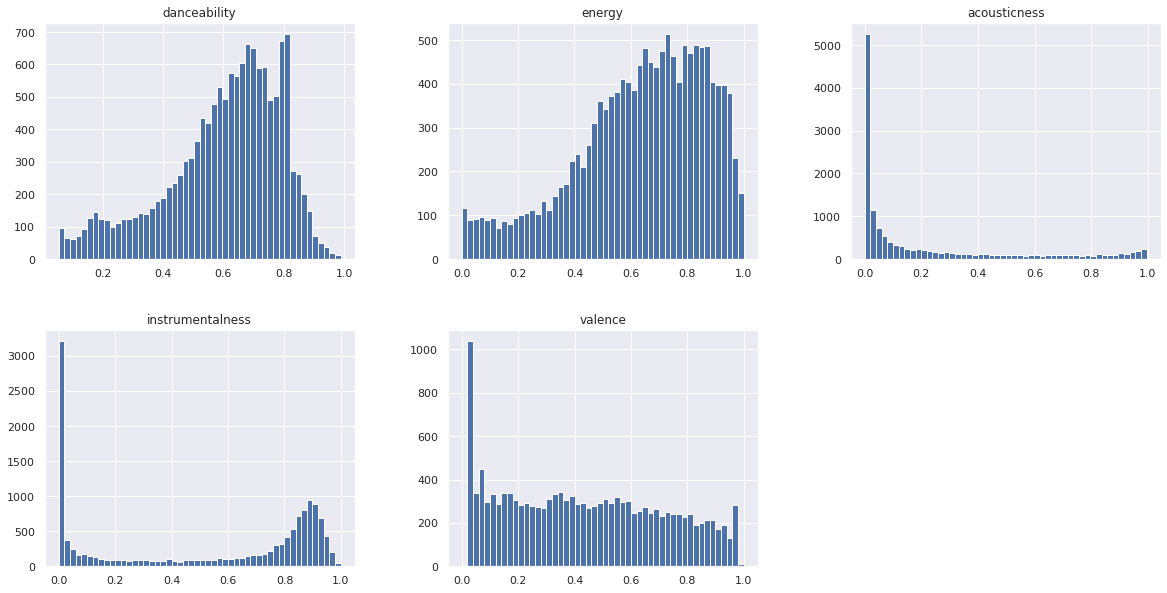
\includegraphics[width=\textwidth]{images/features-distribution.png}
      \caption{Distribution of audio features in the Last.fm Single-user dataset.}
      \label{fig:audio-features-distribution}
\end{figure}

\begin{figure}[h!]
      \centering
      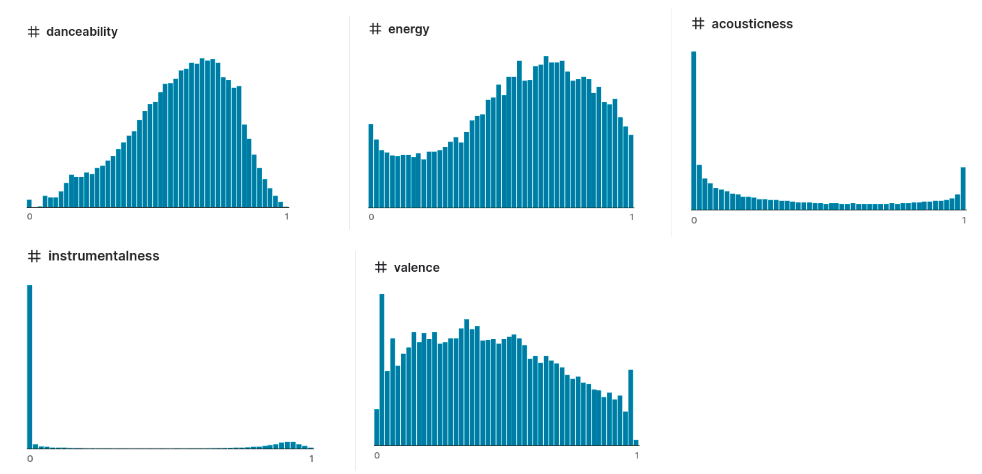
\includegraphics[width=\textwidth]{images/feature-distribution-kaggle.png}
      \caption{Distribution of audio features in the Spotify Audio Features Kaggle dataset.}
      \label{fig:audio-features-distribution-kaggle}
\end{figure}




\section{Experiments}\label{sec5}

We trained three commonly used machine learning models to predict Spotify audio features from Last.fm tags by using the Last.fm Single-user dataset.
Considering that predicting the audio feature values is a regression problem, we tested the following models:

\begin{itemize}
      \item Boosted tree regressor \cite{xgboost}
      \item Bayesian Ridge Regressor \cite{bayesian}
      \item GPT-2 model (fine-tuning) \cite{radford2019language}
\end{itemize}


\subsection{Models}

The \emph{Boosted tree regressor} is a specific implementation of the \emph{XGBoost} algorithm for regression tasks.
This algorithm is an ensemble learning technique that combines simple multiple decision trees to
create a stronger predictive model.
This model has proved to be a powerful solution for classification and regression problems on high-dimensional, structured data.

The \emph{Bayesian Ridge regressor} is a regression model that combines the principles of Bayesian statistics with ridge regression.
Compared to linear regression, which assumes that the model estimated parameters have a deterministic value, the Bayesian Ridge regressor treats the model coefficients as variables with a prior distribution.
By incorporating prior distributions into the learning process, the model is able to capture uncertainty.
The ridge regression technique enables the model to handle noisy, collinear, structured data.

The \emph{GPT-2} model is a transformer model.
Transformers are a type of neural network architecture that has been widely used in natural language processing (NLP) tasks,
such as text generation and question answering.
GPT-2 has been trained on a large corpus of text, and typically used as a language model to generate text that resembles human-written language.
However, in this study we have experimented with GPT-2 as a regressor.
Rather than retraining the model from scratch, we have fine tuned the model to behave as a regressor and  predict Spotify audio features.
The basic idea behind this approach is to feed a string of concatenated Last.fm tags as input to the GPT-2 model, and then use the model's output as the predicted value of a specific Spotify audio feature.

\subsubsection{Models Parametrization}

Due to the different models and input encodings that we employed in the models, we decided to limit the dimensionality of the experiments,
by using mostly the default hyperparameters that the most common libraries set for these models.

For the Bayesian ridge regressor, we used the default hyperparameters set by the \emph{scikit-learn} library.
The training parameters for the Bayesian ridge are listed in table \ref{table_bayesian_training_params}.

To fine tune the GPT-2 model, we used the \emph{GPT2ForSequenceClassification} model of the \emph{Transformers} Python library.
The parameters used are listed in table \ref{table_gpt2_training_params}.

\begin{table}[!ht]
      \begin{minipage}{.5\linewidth}
            \caption{Training parameters for Bayesian Ridge regressor}\label{table_bayesian_training_params}%
            \centering
                  \begin{tabular}{@{}ll@{}}
                  \toprule
                  Parameter                     & Value \\
                  \midrule
                  Maximum iterations            & 300   \\
                  Tolerance\footnotemark[1]     & \num{1e-03} \\
                  alpha 1                       & \num{1e-06} \\
                  alpha 2                       & \num{1e-06} \\
                  lambda 1                      & \num{1e-06} \\
                  lambda 2                      & \num{1e-06} \\
                  \botrule
                  \end{tabular}
            \footnotetext[1]{Tolerance for the stopping criteria.}
            \caption{Training parameters for GPT-2 regressor}\label{table_gpt2_training_params}%
            \centering
                  \begin{tabular}{@{}ll@{}}
                  \toprule
                  Parameter                     & Value \\
                  \midrule
                  Batch size                    & 10 \\
                  Problem type                  & regression \\
                  Epochs                        & 10 \\
                  Sequence length (tokens)      & 256 \\
                  Tokenizer                     & GPT-2 tokenizer \\
                  \botrule
                  \end{tabular}
      \end{minipage}
      \begin{minipage}{.5\linewidth}
            \caption{Training parameters for XGBoost regressor}\label{table_xgboost_training_params}%
            \centering
                  \begin{tabular}{@{}ll@{}}
                  \toprule
                  Parameter               & Value \\
                  \midrule
                  objective               & reg:squarederror  \\
                  base score              & 0.5 \\
                  booster                 & gbtree  \\
                  colsample bylevel       & 1 \\
                  colsample bynode        & 1 \\
                  colsample bytree        & 1 \\
                  gamma\footnotemark[1]   & 0 \\
                  learning rate           & 0.3 \\
                  max delta step          & 0 \\
                  max depth               & 6 \\
                  min child weight        & 1 \\
                  estimators              & 200  \\
                  n jobs                  & 12  \\
                  num parallel tree       & 1 \\
                  predictor               & auto  \\
                  random state            & 0 \\
                  reg alpha               & 0 \\
                  reg lambda              & 1 \\
                  scale pos weight        & 1 \\
                  subsample               & 2 \\
                  tree method             & auto  \\
                  \botrule
                  \end{tabular}
            \footnotetext[1]{Tolerance for the stopping criteria.}
      \end{minipage}
\end{table}


Similarly, for the boosted tree regressor, we used the default parameters set in the \emph{xgboost} Python library.
We configured the boosted tree regressor model with the training parameters listed in table \ref{table_xgboost_training_params}.

\subsection{Last.fm Tags Input Format}

\textcolor{red}{TODO: Create diagram}

The preceding models require specific input formats.
In particular, the boosted tree and bayesian ridge regressors require structured data (e.g a set of predictor features and a set of target variables), whereas GPT-2 expects text strings as input.

Each individual sample in the Last.fm singe-user dataset corresponds to a unique track,
and contains the list of Last.fm tag-count tuples (e.g. \verb|[(electronic, 100), (dance, 45), ...]|)
and the values of Spotify audio features.
The Last.fm single-user dataset was converted to the formats described in the following sections, and then fed into the corresponding models.


\subsubsection{Last.fm Tags as Table Columns}
The tabular format represents the Last.fm tags as columns in a table.
Each tag is defined by a column and each cell contains the count value of a tag for a track.
If a $tag$ is not present for a particular $track$, then cell $c_{track,tag}$ is \num{0}.

Counting the total amount of Last.fm tags in the user collection resulted, initially, in more than five million tags.
Under this high-dimensionality scenario, building a tabular data set, in which every row contains millions of columns (i.e. Last.fm tags) was theoretically possible, but presented scalability problems.
In addition to scalability limitations, classic machine learning models might not take advantage of using the full collection of tags present in the user history.
These models might even perform poorly if too many input features are provided.
The reason for this is spurious relations or redundancy  between input features.
Models might find relations that are not real, and latent, redundant variables might be accountable multiple times, which can lead to a biased outputs.
Feature subject selection aims at solving these problems.


Therefore, we reduced the number of tags by picking a subset of the most relevant tags.
We used a the feature selection algorithm by using a basic data aggregation algorithm: grouping the data by tag, aggregating by summing the \emph{count} values for each tag,
ordering by the aggregated count, and finally selecting the top-$K$ tags of the ranking.
Three values of $K$, were used, thus generating three subsets: \num{100}, \num{1000}, and \num{10000}.
We consider this reduction approach an initial approach approach in our experiments.
For this particular aspect, dimensionality reduction algorithms, such as PCA, are good candidates for future work.

After selecting the top-$K$ tags, the Last.fm single-user dataset was formatted as follows:

\begin{itemize}
      \item Given that $Tags_{K}$ is the set of most $K$ frequent Last.fm tags in the user listening history
            , where each $tag \in Tags_{K}$.
      \item Given that $Audio$ is the set of Spotify audio features, where each $feat \in Audio$.
      \item For each $track$:
      \begin{itemize}
            \item $X_{tag,track}$ is the $count$ value of $tag$ for $track$. This value is in the $0-100$ range.
            \item $y_{track},_{feature}$ is the value of the audio feature $y$ for $track$.
      \end{itemize}
\end{itemize}

An example of this data format is provided in table \ref{tabular_tags_format}.

\begin{table}[h]
      \begin{center}
      \begin{minipage}{\textwidth}
      \caption{Tabular data format for Last.fm tags in XGBoost and Bayesian regressors}\label{tabular_tags_format}%
      \begin{tabular}{@{}lllllll@{}}
      \toprule
      Track                         & $X_{electronic}$ & $X_{ambient}$ & $X_{\dots}$ & $y_{energy}$ & $y_{valence}$ & $y_{\dots}$ \\
      \midrule
      Massive Attack - Blue Lines   & 62               & 6             &  \dots      & 0.496        & 0.947         & \dots  \\
      The Beta Band - Squares       & 40               & 3             &  \dots      & 0.446        & 0.507         & \dots  \\
      \dots                         & \dots            & \dots         &  \dots      & \dots        & \dots         & \dots  \\
      \botrule
      \end{tabular}
      \end{minipage}
      \end{center}
\end{table}

The main drawback of this representation is data sparsity.
For most of the tracks, many columns are \num{0}.

This format was tested with the Bayesian Ridge and the Boosted Tree regressors.

% The sparsity of a matrix is the number of zero-valued elements divided by the total number of elements
% (e.g., m * n for an m * n matrix) is called the sparsity of the matrix.


\subsubsection{Tokens as Table Columns}

This format is also structured, but the input data is a set of tokens instead of tag count values.
These \emph{tokens} are the result of passing the tags, concatenated as a string, through a tokenizer.
Tokenizers are crucial elements in the preprocessing of text data.
A tokenizer dissects a piece of text into smaller units, called tokens.
These tokens can be words, subwords, or even characters.

% Tags are converted to text tokens. Columns represent token positions, and cells contain the token at a particular position, for a track.
% To tokenize tags, we have used the GPT-2 tokenizer.

When breaking down the text into tokens, the tokenizer assigns a unique numerical identifier to each token.
These identifiers are based on the vocabulary that the tokenizer has been trained on.
For example, when the tokenizer processes the \verb|"pop rock"| string, the \verb|pop| token might be assigned to ID \verb|123|
and the \verb|rock| token might be assigned to ID \verb|34534|.
Consequently, the result of tokenizing \verb|pop rock| would be \verb|[123, 34534]|.

Note that, although tokenizers are most commonly used in combination with transformer models, in this paper we test the possibility of using a tokenizer to preproccess the data passed to the models that require structured data.

Because the tokenizer requires a string as the input, we converted the set of tags for each track into a string, in a process that we called \emph{stringification}.
To \emph{stringify} the tags, we concatenated Last.fm tags by following these three strategies:

\begin{itemize}
      \item Order by count: \verb|"rock, pop"|.
      \item Include tag count: \verb|"rock 2, pop 1"|.
      \item Duplicate tags $count$ times: \verb|"rock rock, pop"|.
\end{itemize}


In this particular case, the $X$ values of the tabular input data are the token IDs.
These tokens are obtained from passing the string of concatenated Last.fm tags through the GPT-2 tokenizer,
as the following procedure explains:

\begin{itemize}
      \item Given that $S$ is the stringification strategy.
      \item Given that $X_L$ is the token vocabulary, where $L$ is the maximum vocabulary length.
      \item Given that $Audio$ is the set of Spotify audio features, where each $feat \in Audio$.
      \item For each $track$ and $S$:
      \begin{itemize}
            \item $tags_{track,str}$ is the string of concatenated tags produced by strategy $S$.
            \item $tokens_{track}$ is the list of token IDs produced after tokenizing $tags_{str}$.
            \item $X_{n,track}$ is token ID found at position $n$ of $tokens_{track}$.
            \item $y_{feature, track}$ is the value of the audio feature $y$ for $track$.
      \end{itemize}
\end{itemize}

An example of this data format is provided in table \ref{tabular_token_format}.

\begin{table}[h]
      \begin{center}
      \begin{minipage}{\textwidth}
      \caption{Tabular data format for tokens in XGBoost and Bayesian regressors}\label{tabular_token_format}%
      \begin{tabular}{@{}llllllll@{}}
      \toprule
      Track                         & $X_{0}$ & $X_{1}$ & $X_{2}$ & $X_{\dots}$ & $y_{energy}$ & $y_{valence}$ & $y_{\dots}$ \\
      \midrule
      Massive Attack - Blue Lines   & 101     & 5099    & 6154    &  \dots      & 0.496        & 0.947         &  \dots  \\
      The Beta Band - Squares       & 101     & 4522    & 2600    &  \dots      & 0.446        & 0.507         &  \dots  \\
      \dots                         & \dots   & \dots   & \dots   &  \dots      & \dots        & \dots         &  \dots  \\
      \botrule
      \end{tabular}
      \end{minipage}
      \end{center}
\end{table}

Similarly to the tags tabular format, we also defined fixed values for the number of columns: 10, 1,000, and 10,000.
\textcolor{red}{Describe the name of this particular limit (maxsequence length?)}


Similar to the previous structured format, this format was also used in the Bayesian and Boosted Tree regressors.
In contrast to the previous format, this format does not present sparsity.
It incorporates however, other problems, such as the lack of normalization of the values, which do not represent scalars, but IDs.
It is also harder to inspect, because the meaning of each token is unknown.


\subsubsection{Text Strings}

When using transformer models, the input data is a string.
To use GPT-2, we had to represent the Last.fm tags, which are defined as $(tag, count)$ tuples, as strings.
To this end, we applied the same three transformations used in the tabular tokens formats,
concatenate the tags by ordering by count, by including the tag count, and by duplicating the tags.

After converting to a string, the formal definition of the input data is as follows:

\begin{itemize}
      \item Given that $X$ is tags represented as text.
      \item Given that $Audio$ is the set of Spotify audio features, where each $feat \in Audio$.
      \item For each $track$:
      \begin{itemize}
            \item $X_{track},_{n}$ is set of tags for $track$, encoded as a single string.
            \item $y_{track},_{feature}$ is the value of the audio feature $y$ for $track$.
      \end{itemize}
\end{itemize}

An example of this data format is provided in table \ref{text_format}.

\begin{table}[h]
      \begin{center}
      \begin{minipage}{\textwidth}
      \caption{Text data format for GPT-transformer. In this particular case, the tags have been concatenated by ordering by tag count}\label{text_format}%
      \begin{tabular}{@{}lllll@{}}
      \toprule
      Track                         & $X$                                   & $y_{energy}$ & $y_{valence}$ & $y_{\dots}$ \\
      \midrule
      Massive Attack - Blue Lines   & "hip hop, chill, bristol, \dots"      & 0.496        & 0.947         & \dots  \\
      The Beta Band - Squares       & "alternative rock, folk, \dots"       & 0.446        & 0.507         & \dots \\
      \dots                         & \dots                                 & \dots        & \dots         & \dots  \\
      \botrule
      \end{tabular}
      \end{minipage}
      \end{center}
\end{table}


\textcolor{red}{what is the limit on the sequence length here?}


% \subsection{Boosted Tree Regressor}




% \subsection{Naive Bayes Regressor}

% The Naive Bayes Regressor, and in particular, Bayesian Ridge, is the model used for regression in this case.

% % COMMENT copied FROM BayesianRidge source code
% % https://github.com/scikit-learn/scikit-learn/blob/9aaed4987/sklearn/linear_model/_bayes.py#L24
% %
% %     There exist several strategies to perform Bayesian ridge regression. This
% %     implementation is based on the algorithm described in Appendix A of
% %     (Tipping, 2001) where updates of the regularization parameters are done as
% %     suggested in (MacKay, 1992). Note that according to A New
% %     View of Automatic Relevance Determination (Wipf and Nagarajan, 2008) these
% %     update rules do not guarantee that the marginal likelihood is increasing
% %     between two consecutive iterations of the optimization.





\subsection{Experiments Execution and Results}

The experiments tested the three models, and the three values of $K$: \num{100}, \num{1000}, \num{10000}.
In the Bayesian Ridge and Boosted tree regressors, we tested the two structured data formats: tags and tokens as columns.
In the GPT-2 model, we tested the text data format.

For the formats that required the concatenation of tags into text strings, we tested the three different stringification strategies.

The data was split into a training set (\num{8654} samples), a validation set(\num{2164} samples), and a test set (\num{2705} samples).
The quality of the model was evaluated by using the root mean squared error (RMSE).
This metric was computed on the test set.

Table \ref{table:experiment_results} summaries the experiment results.
The table provides RMSE values for each experiment.


% INFO - Training Set: (8654, 14)
% INFO - Validation Set: (2164, 14)
% INFO - Test Set: (2705, 14)

% TRAINING STATS
% Num examples = 8654
% Num Epochs = 10
% Instantaneous batch size per device = 10
% Total train batch size (w. parallel, distributed & accumulation) = 10
% Gradient Accumulation steps = 1
% Total optimization steps = 8660
% Number of trainable parameters = 124441344


\begin{table}[h!]
      \begin{center}
      \begin{minipage}{\textwidth}
      \caption{Experiment results. Cells values correspond to the RMSE value.
      Highlighted values correspond to the best RMSE value achieved by each model, for each variable.}
      \label{table:experiment_results}%
      \begin{tabular}{@{}lllllll@{}}
      \toprule
      M         & Input format                        & Danceab...       & Acoustic...    & Energy          & Valence         & Instrumen... \\
      \midrule
      Base      &                                     & 0.276            & 0.438           & 0.329          & 0.395           & 0.541          \\
      \midrule
      Bayes     & 100 tags\footnotemark[1]            & 0.159            & 0.261           & 0.197          & 0.243           & 0.307          \\
      Bayes     & 1000 tags                           & 0.153            & 0.253           & 0.190          & 0.237           & 0.299          \\
      Bayes     & 10000 tags                          &\textbf{0.152}    &\textbf{0.251}   &\textbf{0.189}  &\textbf{0.236}   &\textbf{0.297}  \\
      Bayes     & 100 tokens D\footnotemark[2]        & 0.307            & 0.307           & 0.238          & 0.281           & 0.383          \\
      Bayes     & 1000 tokens D                       & 0.201            & 0.315           & 0.249          & 0.297           & 0.399          \\
      Bayes     & 10000 tokens D                      & 0.359            & 0.507           & 0.394          & 0.479           & 0.613          \\
      Bayes     & 100 tokens O\footnotemark[3]        & 0.191            & 0.305           & 0.237          & 0.282           & 0.376          \\
      Bayes     & 1000 tokens O                       & 0.237            & 0.343           & 0.276          & 0.339           & 0.428          \\
      Bayes     & 10000 tokens O                      & 0.237            & 0.343           & 0.276          & 0.339           & 0.428          \\
      Bayes     & 100 tokens TC\footnotemark[4]       & 0.191            & 0.304           & 0.236          & 0.281           & 0.380          \\
      Bayes     & 1000 tokens TC                      & 0.202            & 0.320           & 0.247          & 0.248           & 0.404          \\
      Bayes     & 10000 tokens TC                     & 0.234            & 0.341           & 0.274          & 0.321           & 0.430          \\
      \midrule
      Tree      & 100 tags                            & 0.154            & 0.257           & 0.188          & 0.240           & 0.302          \\
      Tree      & 1000 tags                           & 0.149            &\textbf{0.249}   & 0.184          & 0.236           & 0.292          \\
      Tree      & 10000 tags                          &\textbf{0.148}    & 0.250           &\textbf{0.181}  & \textbf{0.235}  &\textbf{0.291}  \\
      Tree      & 100 tokens D                        & 0.274            & 0.274           & 0.212          & 0.256           & 0.330          \\
      Tree      & 1000 tokens D                       & 0.173            & 0.278           & 0.215          & 0.268           & 0.339          \\
      Tree      & 10000 tokens D                      & 0.172            & 0.276           & 0.217          & 0.266           & 0.342          \\
      Tree      & 100 tokens O                        & 0.179            & 0.294           & 0.225          & 0.271           & 0.350          \\
      Tree      & 1000 tokens O                       & 0.182            & 0.294           & 0.224          & 0.270           & 0.353          \\
      Tree      & 10000 tokens O                      & 0.182            & 0.294           & 0.225          & 0.267           & 0.353          \\
      Tree      & 100 tokens TC                       & 0.172            & 0.280           & 0.211          & 0.262           & 0.342          \\
      Tree      & 1000 tokens TC                      & 0.174            & 0.282           & 0.215          & 0.268           & 0.344          \\
      Tree      & 10000 tokens TC                     & 0.175            & 0.281           & 0.214          & 0.270           & 0.345          \\
      \midrule
      GPT       & Duplicated\footnotemark[5]          & 0.157            & 0.244           & 0.193          & 0.245           & 0.322          \\
      GPT       & Ordered\footnotemark[6]             & 0.149            & \textbf{0.237}  & 0.188          & 0.235           & \textbf{0.297}          \\
      GPT       & Tags,Counts\footnotemark[7]         & \textbf{0.145}   & \textbf{0.237}  & \textbf{0.187} & \textbf{0.233}  & 0.301          \\

      \botrule
      \end{tabular}
      \footnotetext[1]{Tags in tabular format. Given $(rock, 3)$, the cell in the $rock$ column contains \verb*|3|.}
      \footnotetext[2]{Duplicated tokens in tabular format. Tags $(rock, 3), (pop, 2)$, are converted to the \verb*|"rock, rock, rock, pop, pop"| string,
      which a tokenizer converts to the list of input tokens (e.g. \verb*|[101,1005,16588,1005,2531, ...]|).
      These tokens are passed to the model in tabular format. Columns are $token_1$, $token_2$, $...$, $token_N$.}
      \footnotetext[3]{Ordered tokens in tabular format. Tags $(rock, 3), (pop, 2)$, are converted to the \verb*|"rock, pop"| string,
      which a tokenizer converts to the list of input tokens (e.g. \verb*|[101,1005,16588,1005,2531, ...]|).
      These tokens are passed to the model in tabular format. Columns are $token_1$, $token_2$, $...$, $token_N$.}
      \footnotetext[4]{Tokens in tabular format from tags and counts. Tags $(rock, 3), (pop, 2)$, are converted to the \verb*|"'rock' 3, 'pop' 2"| string,
      which a tokenizer converts to the list of input tokens (e.g. \verb*|[101,1005,16588,1005,2531, ...]|).
      These tokens are passed to the model in tabular format. Columns are $token_1$, $token_2$, $...$, $token_N$.}
      \footnotetext[5]{String. Given tags $(rock, 3), (pop, 2)$, input is formatted as \verb*|"rock, rock, rock, pop, pop"|.}
      \footnotetext[6]{String. Given tags $(rock, 3), (pop, 2)$, input is formatted as \verb*|"rock, pop"|.}
      \footnotetext[7]{String. Given tags $(rock, 3), (pop, 2)$, input is formatted as \verb*|"'rock' 3, 'pop' 2"|.}
      \end{minipage}
      \end{center}
\end{table}

The Spotify feature that the models had less trouble estimating was the danceability, and the energy.
The instrumentalness, however, was the feature that presented the highest deviations.
Acousticness and valence also presented high RMSE values.

The GPT-2 model was the best model to predict the danceability, with a \num{0.145} RMSE.
The Boosted tree was the best model to predict the instrumentalness, with a RMSE value of \num{0.29}.

In general, the three models performed similarly, with GPT-2 achieving slightly better results in danceability, acousticness, and valence.
The Boosted Tree regressor was the best model to predict energy, and instrumentalness.

The two regressors achieved the best results when using the \emph{Tags as columns} format, mostly with \num{10000} tags.
Interestingly, the Boosted Tree regressor achieved better results with tokens when estimating valence.
Even better results than GPT-2.
In the rest of the features, the regressors worked better with tags as columns.

Using a higher number of predictor variables was not a synonym of lower error values when using tokens a columns.

The Bayesian regressor was a bit more sensitive to changes in tag formatting.
This model tended to work better with data formatted by using the Tag Count stringification method.
The Boosted Tree regressor presented less sensitivity to format changes, although the model generally performed better with the Tags as columns format too.

The Duplicated stringification method consistently performed worse with the GPT-2 transformer model.



\subsubsection{Results for Tabular Data Models}



\begin{figure}[h!]
      \centering
      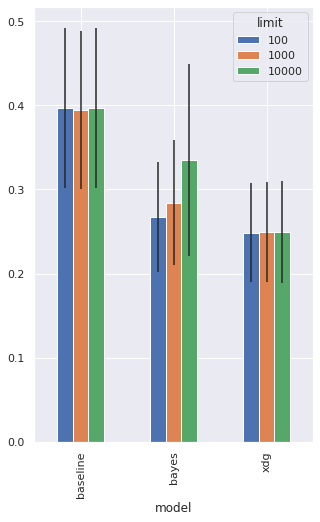
\includegraphics[width=1\textwidth]{images/rmse_by_model_and_limit.png}
      \caption{RMSE mean and standard deviation by model and tags/tokens limit.}
      \label{fig:rmse_by_model_and_limit}
\end{figure}


\begin{figure}[h!]
      \centering
      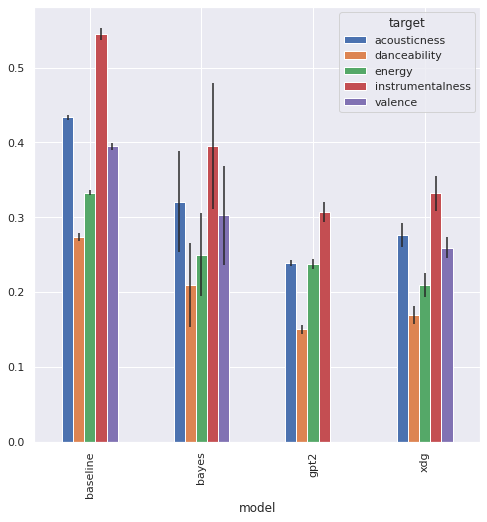
\includegraphics[width=1\textwidth]{images/rmse_by_model_and_feature.png}
      \caption{RMSE mean and standard deviation by model and audio feature.}
      \label{fig:rmse_by_model_and_feature}
\end{figure}


\begin{figure}[h!]
      \centering
      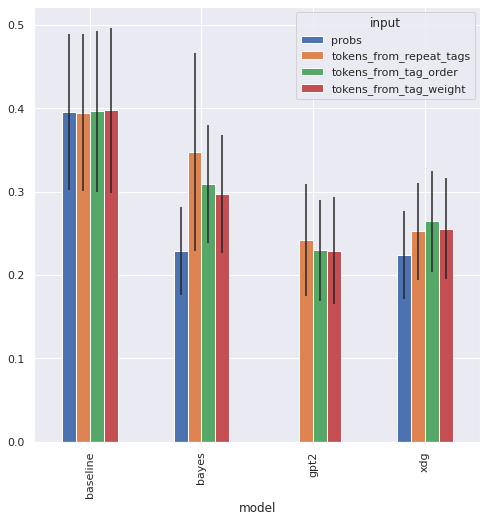
\includegraphics[width=1\textwidth]{images/rmse_by_model_and_input.png}
      \caption{RMSE mean and standard deviation by model and input type (tag probablities or tokens).}
      \label{fig:rmse_by_model_and_input}
\end{figure}


\begin{figure}[h!]
      \centering
      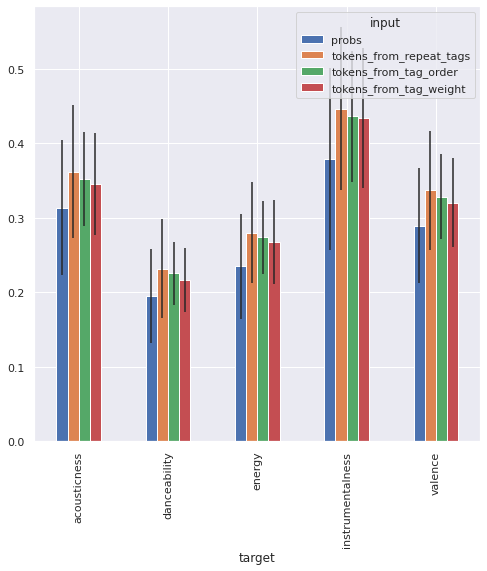
\includegraphics[width=1\textwidth]{images/rmse_by_feature_and_input.png}
      \caption{RMSE mean and standard deviation by audio feature and input type (tag probablities or tokens).}
      \label{fig:rmse_by_feature_and_input}
\end{figure}

\section{Conclusions}\label{sec6}

In general, we believe that this novel approach that has the potential to benefit both listeners and researchers.
By combining subjective user-generated tags with objective audio features,
we can gain new insights into the complex relationship between perception and audio signal in music.

Our approach also presents limitations.
One limitation is the assumption of a strong relationship between Last.fm tags and Spotify features, which may not be true in all cases.
Future work could explore other sources of input values, possibly related to the user context, to improve the accuracy of the predictions.

Track mapping between Last.fm and Spotify is another opportunity for research and improvement.
Although Last.fm provides the MusicBrainz unique identifier, but Spotify does not provide this value.
The mapping was performed by using the track artist and name, but this approach resulted on about 30\% of the tracks not found on Spotify.

The standard deviation values that are displayed in figure \ref{fig:rmse_by_feature_and_input} are in the 0.1-0.2 margin.
Considering this factor, we argue that the RMSE values that some models manifest are, in fact, noteworthy.
For example, the best value for instrumentalness is \num{0.291}.
Considering that the mean and standard deviation for all the experiments with this variable are, respectively,\num{0.414} and\num{0.106}, the z-scores
of \num{0.291} and \num{0.297} are \num{-1.16} and \num{-1.10}.
We can conclude that the \num{0.291} and \num{0.297} values are close to each other and exhibit a similar level of deviation from the mean.

We consider this reduction approach an initial approach approach in our experiments.
For this particular aspect, dimensionality reduction algorithms, such as PCA, are good candidates for future work.


\textcolor{red}{TODO}


\backmatter

\bmhead{Acknowledgments}

This work has been partially funded by the Government of Castilla - La Mancha (SBPLY/21/180225/000062) and by the Spanish Government (PID2019-106758GB-C33 MCIN/AEI/10.13039/501100011033), and also by the UCLM (University of Castilla-La Mancha) and “ERDF A way of making Europe” (2023-GRIN-34437).



%%===========================================================================================%%
%% If you are submitting to one of the Nature Portfolio journals, using the eJP submission   %%
%% system, please include the references within the manuscript file itself. You may do this  %%
%% by copying the reference list from your .bbl file, paste it into the main manuscript .tex %%
%% file, and delete the associated \verb+\bibliography+ commands.                            %%
%%===========================================================================================%%

\bibliography{bibliography}% common bib file
%% if required, the content of .bbl file can be included here once bbl is generated
%%\input sn-article.bbl

%% Default %%
%%\input sn-sample-bib.tex%

\end{document}
